% PRIMARY FIGURE
\begin{figure}[H]
    \centering
    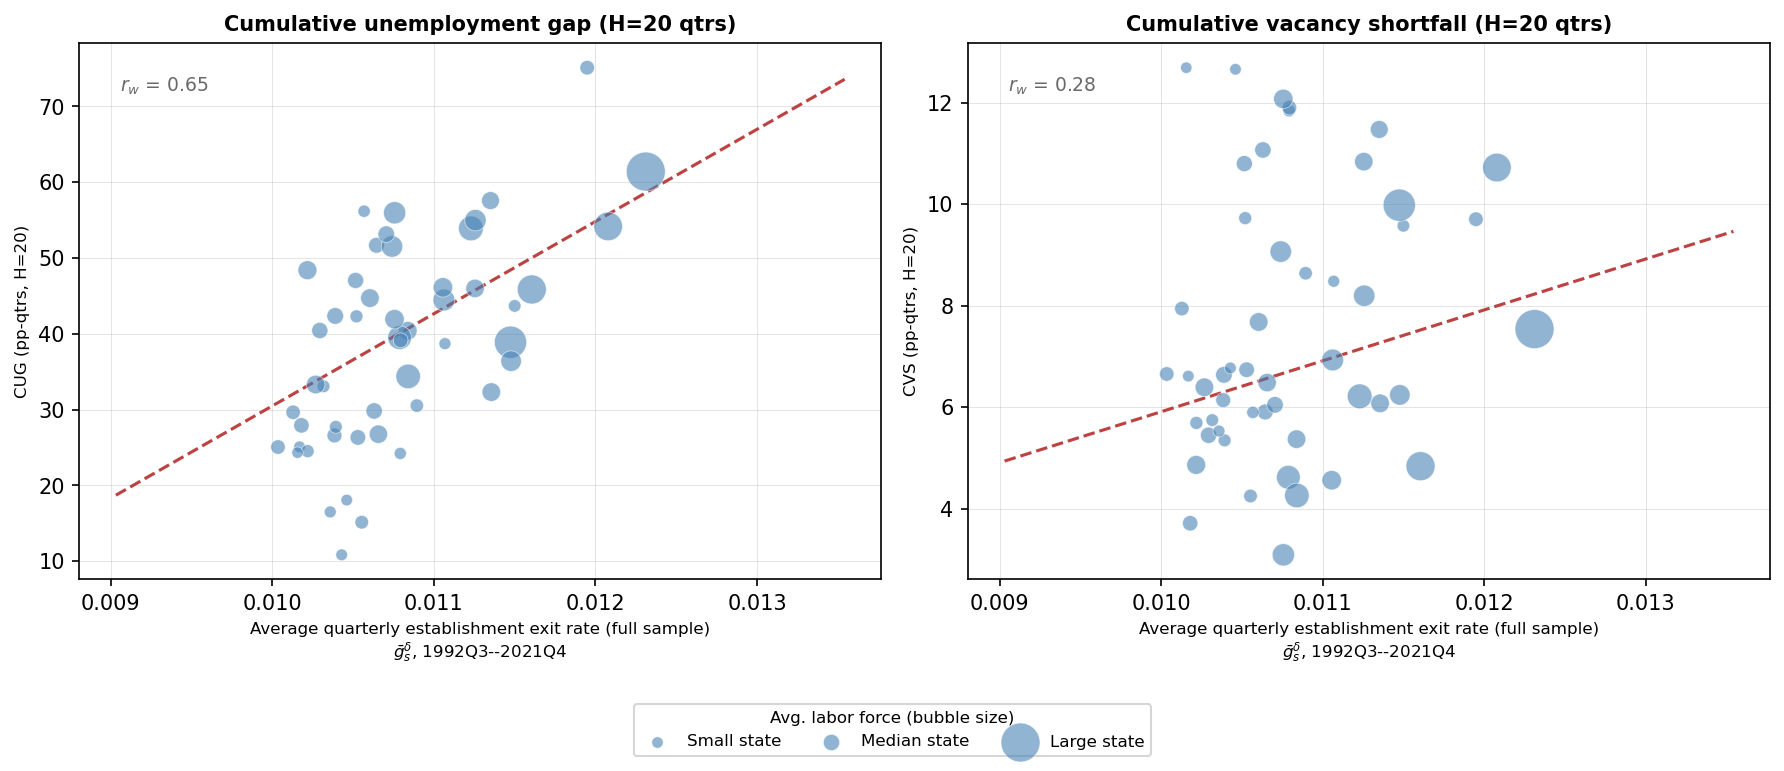
\includegraphics[width=0.92\textwidth]{state_scatter_primary.png}
    \caption{Cross-state relationship between average establishment exit rates
    and cumulative recession labor market damage. Each point is one of the 50
    U.S.\ states; bubble size is proportional to average labor force.
    The horizontal axis is the full-sample time average of the state-level
    Bartik-weighted establishment exit rate ($\bar{g}^\delta_s$,
    1992Q3--2021Q4), constructed from BLS Business Employment Dynamics (BED)
    data using 2006 base-year employment shares.
    The left panel shows the cumulative unemployment gap (CUG): the
    sum of quarterly deviations of the unemployment rate above its
    pre-recession average over $H=20$ quarters from recession onset,
    in percentage-point-quarters. The right panel shows the analogous
    cumulative vacancy shortfall (CVS) for the vacancy rate.
    Both outcomes are averaged across the three post-1992 NBER recessions
    (2001, 2007--2009, 2020), weighted by state labor force at recession onset.
    The regression line is estimated by WLS with state labor force weights;
    $r_w$ denotes the labor-force-weighted correlation.}
    \label{fig:state_scatter}
\end{figure}

% APPENDIX FIGURE
\begin{figure}[H]
    \centering
    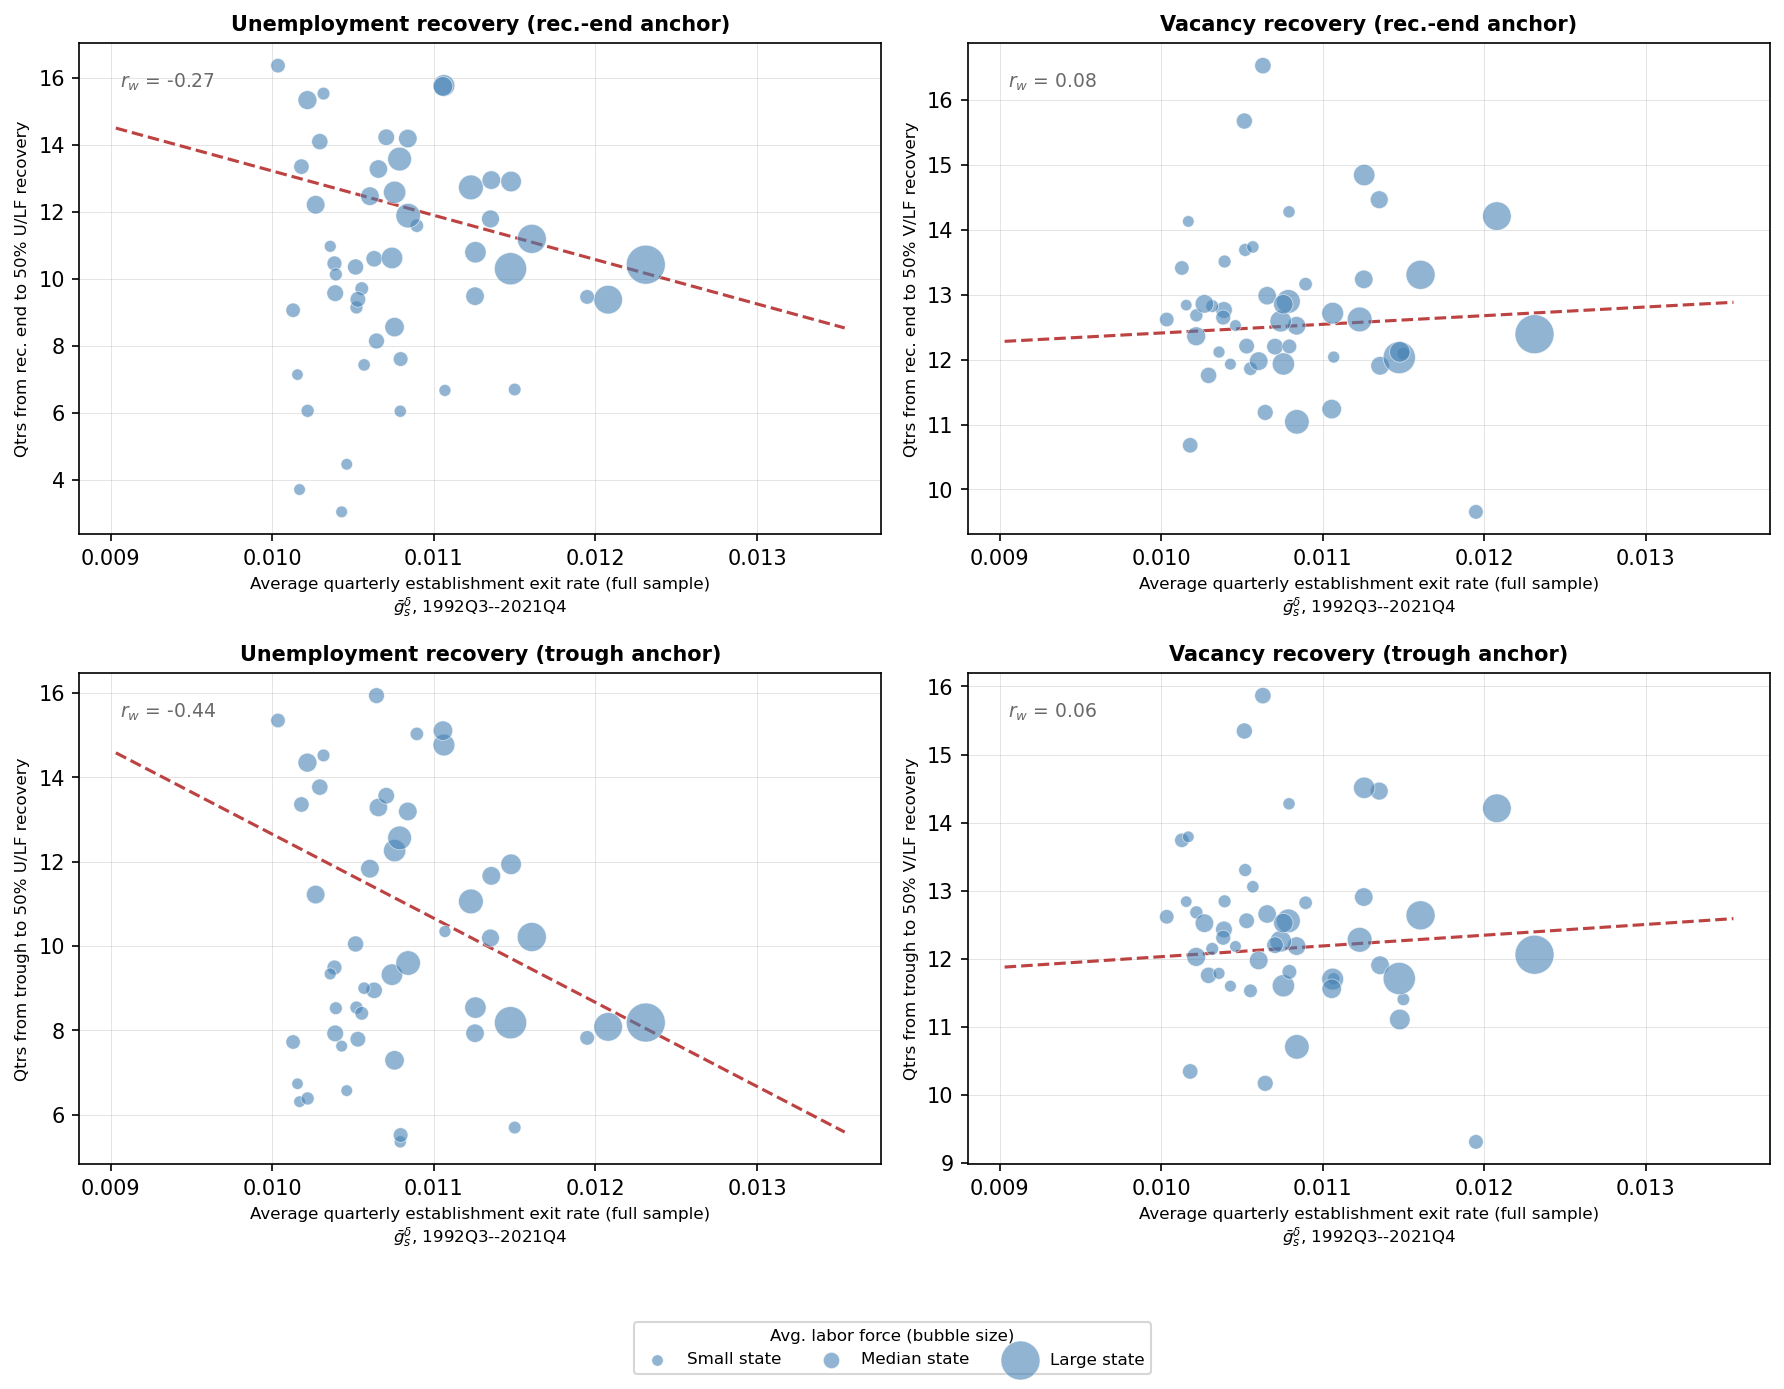
\includegraphics[width=0.92\textwidth]{state_scatter_appendix.png}
    \caption{Cross-state relationship between average establishment exit rates
    and recession recovery speed. Layout and data sources as in
    Figure~\ref{fig:state_scatter}. The top row shows quarters from the NBER
    recession end date until 50\% closure of the trough gap for unemployment
    (left) and vacancy rates (right); the bottom row uses the series trough
    date as the clock origin. Recovery speed does not exhibit a robust positive
    relationship with exit rates in the cross-section, reflecting compositional
    differences in industry structure across high- and low-exit-rate states.
    The cumulative gap measures in Figure~\ref{fig:state_scatter} provide the
    cleaner cross-state comparison.}
    \label{fig:state_scatter_appendix}
\end{figure}
